\documentclass[fleqn, a4paper, 12pt, twoside]{article}
\usepackage{exsheets} %question and solution environments
\usepackage{amsmath, amssymb, amsthm} %standard AMS packages
\usepackage{esint} %integral signs
\usepackage{marginnote} %marginnotes
\usepackage{gensymb} %miscellaneous symbols
\usepackage{commath} %differential symbols
\usepackage{xcolor} %colours
\usepackage{cancel} %cancelling terms
\usepackage[free-standing-units]{siunitx} %formatting units
\usepackage{tikz, pgfplots} %diagrams
	\usetikzlibrary{calc, hobby, patterns, intersections, angles, quotes, spy}
\usepackage{graphicx} %inserting graphics
\usepackage{epstopdf} %converting and inserting eps graphics
\usepackage{hyperref} %hyperlinks
\usepackage{datetime} %date and time
\usepackage{ulem} %underline for \emph{}
\usepackage{xfrac, lmodern} %inline fractions
\usepackage{enumerate, enumitem} %numbered lists
\usepackage{float} %inserting floats
\usepackage[american voltages]{circuitikz} %circuit diagrams
\usepackage{pdflscape} %pages in landscape orientation
\usepackage{setspace} %double spacing
\usepackage{microtype} %micro-typography
\usepackage{listings} %formatting code
	\lstset{language=Matlab}
	\lstdefinestyle{standardMatlab}
	{
		belowcaptionskip=1\baselineskip,
		breaklines=true,
		frame=L,
		xleftmargin=\parindent,
		language=C,
		showstringspaces=false,
		basicstyle=\footnotesize\ttfamily,
		keywordstyle=\bfseries\color{green!40!black},
		commentstyle=\itshape\color{purple!40!black},
		identifierstyle=\color{blue},
		stringstyle=\color{orange},
	}
\usepackage{algpseudocode} %algorithms
\usepackage{algorithm} %algorithms
\usepackage{chronology}
\usepackage{qtree}
\usepackage{varwidth}

\newcommand\numberthis{\addtocounter{equation}{1}\tag{\theequation}} %adds numbers to specific equations in non-numbered list of equations

\theoremstyle{definition}
\newtheorem{example}{Example}
\newtheorem{definition}{Definition}

\theoremstyle{theorem}
\newtheorem{theorem}{Theorem}
\newtheorem{law}{Law}

\newcommand{\curl}{\mathrm{curl\,}}

\newcommand{\divergence}{\mathrm{div\,}}

\makeatletter
\@addtoreset{section}{part} %resets section numbers in new part
\makeatother

\newcommand\blfootnote[1]{%
	\begingroup
	\renewcommand\thefootnote{}\footnote{#1}%
	\addtocounter{footnote}{-1}%
	\endgroup
}

\renewcommand{\tilde}{\widetilde}

\SetupExSheets{solution/print = true} %prints all solutions by default

%opening
\title{Quantum and Solid State Physics}
\author{Aakash Jog}
\date{2015-16}

\begin{document}

\maketitle
%\setlength{\mathindent}{0pt}

\blfootnote
{	
	\begin{figure}[H]
		
\includegraphics[height = 12pt]{cc.eps}
		\includegraphics[height = 12pt]{by.eps}
		\includegraphics[height = 12pt]{nc.eps}
		\includegraphics[height = 12pt]{sa.eps}
	\end{figure}
	This work is licensed under the Creative Commons Attribution-NonCommercial-ShareAlike 4.0 International License. To view a copy of this license, visit \url{http://creativecommons.org/licenses/by-nc-sa/4.0/}.
} %CC-BY-NC-SA license

\tableofcontents

\newpage
\part{Quantum Physics}

\newpage
\part{Solid State Physics}

\section{Lecturer Information}

\textbf{Tammy Ben-Yaacov}\\
~\\
E-mail: \href{mailto:tammybenyaacov@gmail.com}{tammybenyaacov@gmail.com}\\

\section{Required Reading}

\begin{enumerate}
	\item Griffiths, D. Introduction to quantum mechanics
	\item Streetman, B. Solid State Electronic Devices
\end{enumerate}

\section{Additional Reading}

\begin{enumerate}
	\item Kittel, Introduction to solid state physics, John Wiley \& Sons.
	\item Tang: Fundamentals of quantum mechanics, Cambridge press.
	\item Miller, Quantum mechanics for scientists and engineers.
	\item Pierret. Advanced semiconductor Fundamentals, Prentice Hall.
	\item Ashcroft, Solid State Physics, Harcourt college publishers.
\end{enumerate}

\section{Electrons}

\begin{definition}[Particle nature of electrons]
	An electron behaves as a negatively charged charge carrying particle.\\
	The magnitude of the charge on it is
	\begin{align*}
		q & = 1.602 \times 10^{-19} \coulomb
	\end{align*}
	Its mass is
	\begin{align*}
		m_0 & = 9.11 \times 10^{-31} \kilogram
	\end{align*}
\end{definition}

\begin{definition}[Wave nature of electrons]
	Electrons exhibit wave-like properties, in addition to particle-like properties.\\
	The energy transmitted by a wave is
	\begin{align*}
		E & = h \nu \\
                  & = \frac{h c}{\lambda}
	\end{align*}
	where
	\begin{align*}
		h       & = \text{Planck's constant} \left( 6.626 \times 10^{-34} \right) \\
		\nu     & = \text{frequency}                                              \\
		c       & = \text{speed of light}                                         \\
		\lambda & = \text{wavelength}
	\end{align*}
\end{definition}

\section{Semiconductors}

\begin{law}[Ohm's Law]
	The voltage across two points on a conductor is directly proportional to the current through the conductor.
	The constant of proportionality is called the resistance of the conductor.
	\begin{equation*}
		\frac{V}{I} = R
	\end{equation*}
	\label{Ohm's_Law}
\end{law}

\begin{law}[Microscopic Ohm's Law]
	\begin{equation*}
		\overrightarrow{J} & = \sigma \overrightarrow{E}
	\end{equation*}
	where $\overrightarrow{J}$ is the current density, $\sigma$ is the conductivity, $\overrightarrow{E}$ is the electric field in the resistor.
	\label{Microscopic_Ohm's_Law}
\end{law}

\begin{definition}[Resistivity]
	If
	\begin{equation*}
		R = \rho \frac{L}{A}
	\end{equation*}
	where $R$ is the resistance of the resistor, $L$ is the length of the resistor, and $A$ is the cross-sectional area of the resistor, then $\rho$ is called the resistivity of the resistor.\\
	$\sigma = \frac{1}{\rho}$ is called the conductivity of the resistor.\\
	They are constant for a particular material.
\end{definition}

\begin{figure}[H]
	\begin{tikzpicture}
		\begin{scope}
			\draw [green] (0,0) -- (3,0);
			\draw [yellow] (3,0) -- (6,0);
			\draw [-stealth, red] (6,0) -- (9,0);
			\node [right] at (9,0) {$\rho$};
		\end{scope}

		\begin{scope}
			\draw ($ (3,0) + (0,0.1) $) -- ($ (3,0) + (0,-0.1) $) node [below] {$10^{-5}$};

			\draw ($ (6,0) + (0,0.1) $) -- ($ (6,0) + (0,-0.1) $) node [below] {$10^6$};
		\end{scope}

		\begin{scope}
			\node [above] at (1.5,0) {Conductors};
			\node [above] at (4.5,0) {Semiconductors};
			\node [above] at (7.5,0) {Insulators};
		\end{scope}
	\end{tikzpicture}
\end{figure}

\subsection{Control Factors}

The major factors which affect the conductivity of a material are

\begin{enumerate}
	\item Temperature
	\item Chemical composition
		\begin{enumerate}
			\item Atomic bonding
			\item Crystal structure
			\item Charge carriers in the crystal
		\end{enumerate}
	\item Optical effects
	\item Doping
\end{enumerate}

\subsection{Chemical Makeup}

\begin{table}[H]
	\begin{tabular}{c|c|c|c|c}
		\mathrm{II} & \mathrm{III} & \mathrm{IV} & \mathrm{V} & \mathrm{VI} \\
		\hline
	                    & B            & C           & N          & O           \\
	                    & Al           & Si          & P          & S           \\
		Zn          & Ga           & Ge          & As         &             \\
		Cd          & In           &             &            &             \\
	\end{tabular}
\end{table}

\begin{enumerate}
	\item Easily available, hence economical
	\item Performs better at higher temperatures
	\item Can be converted to silica on heating
\end{enumerate}

\begin{figure}[H]
	\Tree
	[
		.Semiconductors
		[
			.Elemental
		]
		[
			.Compound
			[
				.{Binary Compound SCs}
				[
					.{$\mathrm{III}$-$\mathrm{V}$}
					{
						GaAs, InP, GaN
					}
				]
				[
					.{$\mathrm{II}$-$\mathrm{VI}$}
					{
						ZnO
					}
				]
			]
			[
				.{Ternary Compound SCs}
				{
					AlGaAs, InGaN
				}
			]
		]
	]
	\caption{Classification of Semiconductors}
\end{figure}

\begin{question}
	A sample of Germanium has resistivity $\rho = 0.46 \ohm\metre$.
	The dimensions of the sample are
	\begin{align*}
		l & = 50 \si{\micro\metre}  \\
		h & = 0.2 \si{\micro\metre} \\
		w & = 1 \si{\micro\metre}
	\end{align*}
	Find the resistance of the sample and the conductivity of the material.
\end{question}

\begin{solution}
	\begin{align*}
		\rho & = 0.46 \si{\ohm\metre} \\
                     & = 46 \si{\ohm\centi\metre}
	\end{align*}
	Therefore,
	\begin{align*}
		\sigma & = \frac{1}{\rho}                     \\
                       & = \frac{1}{46 \si{\ohm\centi\metre}} \\
                       & = 0.022 \si{\per \ohm \per \centi\metre}
	\end{align*}
	Therefore,
	\begin{align*}
		l & = 50 \micro\metre \\
                  & = 50 \times 10^{-4} \centi\metre
	\end{align*}
	Therefore,
	\begin{align*}
		R & = \rho \frac{l}{A} \\
                  & = 11500 \times 10^{-4} \ohm
	\end{align*}
\end{solution}

\begin{question}
	A sample of Germanium has resistivity $\sigma$.
	The dimensions of the sample are as shown.
	\begin{figure}[H]
		\begin{tikzpicture}
			\def\C{3};
			\def\L{5};
			\def\B{2};
			\def\W{1};

			\begin{scope}
				\draw (0,0) -- (\L,0) -- (\L,\B) -- (0,\C) -- cycle;
				\draw [xshift = \W cm, yshift = \W cm] (0,0) -- (\L,0) -- (\L,\B) -- (0,\C) -- cycle;

				\draw (0,0) -- ++(\W,\W);
				\draw (\L,0) -- ++(\W,\W);
				\draw (\L,\B) -- ++(\W,\W);
				\draw (0,\C) -- ++(\W,\W);
			\end{scope}

			\begin{scope}[stealth-stealth]
				\draw [xshift = -10] (0,0) -- (0,\C) node [midway, left] {$C$};
				\draw [yshift = -10] (0,0) -- (\L,0) node [midway, below] {$L$};
				\draw [xshift = 10] ($ (\L,0) + (\W,\W) $) -- ($ (\L,\B) + (\W,\W) $) node [midway, right] {$B$};
				\draw [xshift = 10, yshift = -10] (\L,0) -- ++(\W,\W) node [midway, below right] {$W$};
			\end{scope}
		\end{tikzpicture}
	\end{figure}
	Find the relationship between $R$ and $\sigma$.
\end{question}

\begin{solution}
	Consider a slice with height $h$, width $w$, and thickness $\dif x$.
	Therefore, the cross-sectional area of the elemental slice is
	\begin{align*}
		\dif A & = w h                                    \\
                       & = w \left( \frac{B - C}{L} x + C \right) \\
                       & = w \left( \frac{B x - C (L - x)}{L} \right)
	\end{align*}
	Therefore,
	\begin{align*}
		\dif R & = \frac{\dif x}{\sigma w h} \\
                       & = \frac{L \dif x}{\sigma w \left( B x - C (L - x) \right)}
	\end{align*}
\end{solution}

\section{Types of Materials}

Atoms tend to arrange themselves in such a way that the resultant energy is minimized.

\begin{figure}[H]
	\Tree
	[
		.Materials
		[
			.Amorphous
			{
				\begin{varwidth}{4cm}
					No well-defined structure
				\end{varwidth}
			}
		]
		[
			.Polycrystalline
			{
				\begin{varwidth}{4cm}
					Many small regions, each having well organized atomic structure
				\end{varwidth}
			}
		]
		[
			.Crystalline
			{
				\begin{varwidth}{4cm}
					Long range 3D order of atoms, with repeating unit cells, throughout the entire solid
				\end{varwidth}
			}
		]
	]
	\caption{Classification of Materials}
\end{figure}

Semiconductor devices can use all of these types of materials.\\
\begin{figure}[H]
	\begin{tikzpicture}
		\def\h{2};
		\def\l{6};

		\begin{scope}
			\draw (0,0) rectangle ++(\l,\h);

			\node [left] at (0,\h/2) {$S$};

			\node at (\l/2,\h/2) {Si substrate (crystalline)};
		\end{scope}

		\begin{scope}[yshift = \h cm]
			\draw (0,0) rectangle ++(\l,\h);

			\node [left] at (0,\h/2) {$O$};

			\node at (\l/2,\h/2) {SiO$_2$ (amorphous)};
		\end{scope}

		\begin{scope}[yshift = 2*\h cm]
			\draw (0,0) rectangle ++(\l,\h);

			\node [left] at (0,\h/2) {$M$};

			\node at (\l/2,\h/2) {poly Si (polycrystalline)};
		\end{scope}
	\end{tikzpicture}
	\caption{MOS which uses all three types of materials}
\end{figure}

\section{Bohr's Model}

According to Bohr's model of the atom, electrons can have discrete energy levels only.
The electrons in an atom are arranged in the order of filling electronic shells, given by the Aufbau Principle.\\
The energy of a free electron is called $E_{\textnormal{vac}}$.
This is used as a reference energy.

\end{document}
